\section{Method: FinSTaR}
\label{sec:method}

We train FinSTaR via supervised fine-tuning (SFT) on FinTSR-Bench data with structurally different chain-of-thought supervision for 1) assessment tasks and 2) prediction tasks.

\textbf{Why two CoT strategies?}
Assessment and prediction tasks have fundamentally different epistemological properties.
Assessment tasks (e.g., ``What is the current drawdown?'') have answers that are \textit{fully determined} by the observable price data, and the model simply needs to compute the right quantity.
Prediction tasks (e.g., ``Will this drawdown recover?'') have answers that depend on \textit{future events} influenced by unobservable factors such as earnings surprises.
%, macroeconomic shifts, or institutional flows.
Even with a perfect model, prediction accuracy cannot reach 100\% because the necessary information is not contained in the price history alone.
This fundamental distinction between \textit{deterministic} and \textit{probabilistic} reasoning motivates our design of two complementary CoT strategies tailored to each reasoning mode: Compute-in-CoT for \textit{deterministic} assessment and Scenario-Aware CoT for \textit{stochastic} prediction.

\subsection{Compute-in-CoT (Assessment Tasks)}

For assessment tasks, the answer is deterministically computable from observable prices. We generate CoT chains programmatically by executing the same computation the model should learn. Each chain follows a three-phase structure (Figure~\ref{fig:cot_examples}a):
\begin{enumerate}[leftmargin=1.8cm, labelsep=0.3cm]
\item[\textbf{Phase 1.}] \textbf{Extract}: Identify relevant quantities from input prices (e.g., peak price, recent returns).
% \item[\textbf{Phase 2.}] \textbf{Compute}: Perform the necessary calculation (e.g., drawdown percentage, volatility ratio).
\item[\textbf{Phase 2.}] \textbf{Compute}: Perform the calculation (e.g., drawdown percentage, volatility ratio).
% \item[\textbf{Phase 3.}] \textbf{Classify}: Map the computed result to the answer using the thresholds stated in the question.
\item[\textbf{Phase 3.}] \textbf{Classify}: Map the computed result to the answer using the thresholds in the question.
\end{enumerate}
This guarantees 100\% correctness and unlimited scalability, as models never reference unobservable information at inference time.


\subsection{Scenario-Aware CoT (Prediction Tasks)}
\label{sec:scenario_cot}

For prediction tasks, the answer depends on future outcomes influenced by unobservable factors, 
%where a deterministic CoT would teach the model to be overconfident about inherently uncertain outcomes.
where a \textit{deterministic CoT can be problematic as it may lead the model to be overconfident} about 
%inherently 
uncertain outcomes.
Instead, we propose Scenario-Aware CoT, which teaches the model to consider \textit{multiple scenarios} before making a 
\textit{probabilistic}
judgment.
Each 
%prediction 
CoT follows a five-phase structure:
\begin{enumerate}[leftmargin=1.8cm, labelsep=0.3cm]
\item[\textbf{Phase 1.}] \textbf{Extract}: (Same as assessment) Identify relevant quantities from the data.
\item[\textbf{Phase 2.}] \textbf{Compute}: Calculate price-based features (e.g., drawdown depth, recent momentum).
\item[\textbf{Phase 3.}] \textbf{Scenario Analysis}: Generate three scenarios:
  \begin{itemize}[leftmargin=-0.85cm]
%   \item \textit{Base case}: The most probable outcome given current price patterns and no major external events.
  \item \textit{Base case}: The most probable outcome given current price patterns and no external events.
%   \item \textit{Adverse scenario}: An external shock (e.g., earning miss) that could reverse the expected outcome.
  \item \textit{Adverse scenario}: An external shock that could reverse the expected outcome.
  \item \textit{Favorable scenario}: A positive catalyst that strengthens the expected outcome.
  \end{itemize}
% \item[\textbf{Phase 4.}] \textbf{Assessment}: Consider all scenarios to determine which outcome is most supported by current data.
\item[\textbf{Phase 4.}] \textbf{Assessment}: Consider all scenarios to determine which outcome is most supported.
\item[\textbf{Phase 5.}] \textbf{Judgment}: Select the outcome most supported by the scenario analysis and input data.
\end{enumerate}

\textbf{Scenario templates.}
For each (task, answer) pair, we define domain-specific scenario templates grounded in financial knowledge.
For example, \textit{Volatility Forecast} scenarios reference volatility clustering (base), event-driven spikes (adverse), and market calming (favorable).
During training, the model learns these patterns; at inference, it generates scenario reasoning adapted to the specific input, not template copies (see Section~\ref{sec:analysis}).
Scenario templates for all tasks are provided in Appendix~\ref{app:scenario_templates}.

\textbf{Training setup.}
We fine-tune two backbones via LoRA~\cite{hu2022lora}: TimeOmni-1-7B~\cite{timeomni1}, an LLM trained with TS reasoning SFT and RL on Qwen2.5-7B, and Qwen2.5-7B-Instruct~\cite{qwen2025qwen25}, the same base LLM without TS-specific training.
As shown in Table~\ref{tab:main_results}, these are the best-performing models from their respective categories.
%Both backbones are trained in two modes for ablation: \textbf{w/ CoT} (full reasoning chain supervision with Scenario-Aware CoT for prediction tasks) and \textbf{w/o CoT} (answer-only supervision to measure how much reasoning contributes beyond pattern memorization).
We use LoRA with $r{=}32$, $\alpha{=}64$,
%on all linear layers, 
learning rate $5{\times}10^{-5}$, 4 epochs, batch size 1 with gradient accumulation 16, max sequence length 4096, trained on 2$\times$ NVIDIA L40S GPUs.
Unless otherwise stated, FinSTaR refers to TimeOmni-1-7B fine-tuned with our CoT strategies.

\begin{figure}[t]
\vspace{-32pt}
\centering
\begin{subfigure}[t]{\textwidth}
\centering
\begin{minipage}[c]{0.36\textwidth}
\centering
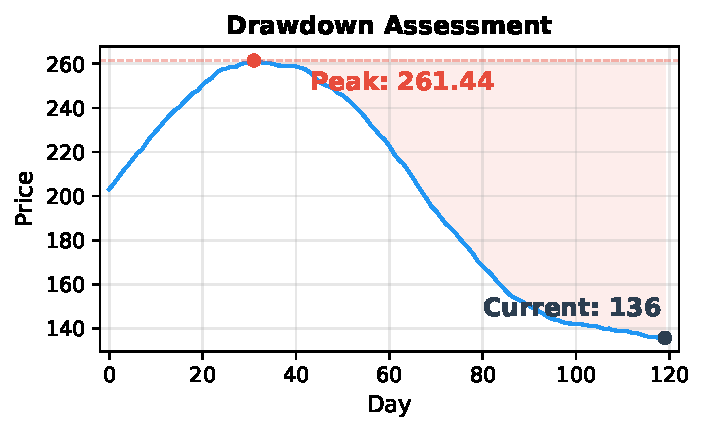
\includegraphics[width=\textwidth]{figures/example_drawdown.pdf}
\end{minipage}
\hfill
\begin{minipage}[c]{0.58\textwidth}
\texttt{\footnotesize Step 1: Peak = 261.44 (day 30).} \\
\texttt{\footnotesize Step 2: Current price = 136.00.} \\
\texttt{\footnotesize Step 3: Drawdown = (261.44$-$136.00)/261.44 = 48.0\%} \\
\hspace*{3.8em}\texttt{\footnotesize 48.0\% $>$ 20\% $\Rightarrow$ (D) Severe Decline ($>$ 20\%).}
\end{minipage}
\vspace{-6pt}
\caption{Simplified example of \textbf{Compute-in-CoT}: Assessment task - Drawdown.}
\label{fig:cot_example_assess}
\vspace{8pt}
\end{subfigure}
\vspace{10pt}
\begin{subfigure}[t]{\textwidth}
\centering
\begin{minipage}[c]{0.36\textwidth}
\centering
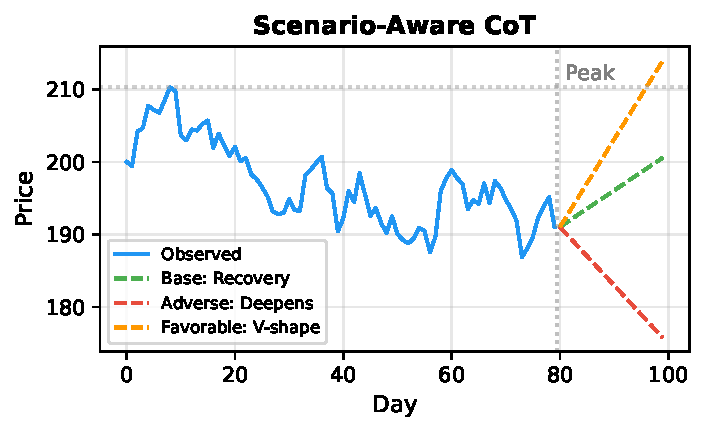
\includegraphics[width=\textwidth]{figures/example_scenario.pdf}
\end{minipage}
\hfill
\begin{minipage}[c]{0.60\textwidth}
\texttt{\footnotesize Step 1: Peak = 210.15 (day 8), Current = 191.08.} \\
\texttt{\footnotesize Step 2: Drawdown = 9.1\%, momentum = $-$2.1\%.} \\
\texttt{\footnotesize Step 3: Scenario analysis:} \\
\hspace*{1.28em}\texttt{\footnotesize $\bullet$ Base: Stabilizes, value buyers $\rightarrow$ recovery.} \\
\hspace*{1.28em}\texttt{\footnotesize $\bullet$ Adverse: Earnings revision $\rightarrow$ decline.} \\
\hspace*{1.28em}\texttt{\footnotesize $\bullet$ Favorable: Upgrade $\rightarrow$ V-shaped recovery.} \\
\texttt{\footnotesize Step 4: Consider all scenarios $\Rightarrow$ recovery.} \\
\texttt{\footnotesize Step 5: Judgment: Recovery $\Rightarrow$ (A).}
\end{minipage}
\vspace{-3pt}
\caption{Simplified example of \textbf{Scenario-Aware CoT}: Prediction task - Drawdown Recovery.}
\label{fig:cot_example_scenario}
\end{subfigure}
\vspace{-20pt}
\caption{\textbf{Two CoT strategies (simplified).} Assessment tasks use Compute-in-CoT that extracts and computes quantities from observable prices. Prediction tasks use Scenario-Aware CoT that generates base/adverse/favorable scenarios before making a judgment. Full examples are in Appendix~\ref{app:tasks}.}
\label{fig:cot_examples}
\vspace{-14pt}
\end{figure}
